\documentclass{article}

\usepackage[utf8]{inputenc}

\usepackage{amsmath, bm}
\usepackage{graphicx}
\usepackage{amssymb}
\usepackage{float}
\usepackage{caption}
\usepackage{subcaption}
\usepackage{hyperref}
\usepackage{tikz}
\usepackage{pgfgantt}
\usepackage{layout}

\usepackage[margin=1in]{geometry}
\usepackage{listings}
\usepackage{xcolor}
\usepackage{color, colortbl}
\usepackage{textgreek}
\usepackage{mathrsfs}
\usepackage{savetrees}

\usetikzlibrary{calc}
\usetikzlibrary{angles,quotes} % for pic
\usetikzlibrary{patterns,snakes}
\usetikzlibrary{arrows}
\usetikzlibrary{shapes.geometric, arrows}
\tikzset{>=latex} % for LaTeX arrow head

\setlength{\parskip}{\baselineskip}%
\setlength{\parindent}{0pt}%
\linespread{0.9}


\definecolor{codegreen}{rgb}{0,0.6,0}
\definecolor{codegray}{rgb}{0.5,0.5,0.5}
\definecolor{codepurple}{rgb}{0.58,0,0.82}
\definecolor{backcolour}{rgb}{0.95,0.95,0.92}

\lstdefinestyle{mystyle}{
    backgroundcolor=\color{backcolour},   
    commentstyle=\color{codegreen},
    keywordstyle=\color{magenta},
    numberstyle=\tiny\color{codegray},
    stringstyle=\color{codepurple},
    basicstyle=\ttfamily\footnotesize,
    breakatwhitespace=false,         
    breaklines=true,                 
    captionpos=b,                    
    keepspaces=true,                 
    numbers=left,                    
    numbersep=5pt,                  
    showspaces=false,                
    showstringspaces=false,
    showtabs=false,                  
    tabsize=2
}
\tikzset{
    cg/.style={
        draw,
        circle,
        thick,
        minimum size=0.2cm, % Adjust the size of the circle
        inner sep=0,      % Remove extra padding
        append after command={
            \pgfextra{
                \draw[thick] (\tikzlastnode.south) -- (\tikzlastnode.north);
                \draw[thick] (\tikzlastnode.west) -- (\tikzlastnode.east);
            }
        }
    }
}

\lstset{style=mystyle}

\tikzstyle{startstop} = [rectangle, rounded corners, minimum width=3cm, minimum height=1cm,text centered, draw=black, fill=red!30]
\tikzstyle{process} = [rectangle, minimum width=3cm, minimum height=1cm, text centered, draw=black, fill=orange!30]
\tikzstyle{decision} = [diamond, minimum width=3cm, minimum height=1cm, text centered, draw=black, fill=green!30]
\tikzstyle{io} = [trapezium, trapezium left angle=70, trapezium right angle=110, minimum width=3cm, minimum height=1cm, text centered, draw=black, fill=blue!30]
\tikzstyle{arrow} = [thick,->,>=stealth]

\begin{document}
\immediate\write18{py mergebib.py}

\title{4F2 Robust and Nonlinear control}
\author{5735G}
\date{Feburary 2025}
\maketitle 

\begin{center}
    \textbf{Summary} \\
    I dont know what to do for this
\end{center}

%-----------------------------------------------------------------------------------------
\section{Motivation}
%-----------------------------------------------------------------------------------------
pass


\section{Application to problem}

The dynamics of a soft link robot can be described by the following equation of motion:

\begin{equation}
    m\ddot{y} + c_v \dot{y} + c_p y = c_p u
\end{equation}

\begin{table}[h]
    \centering
    \begin{tabular}{c|ll|l}
        Variable & Value & Uncertainty & Description \\
        \hline
        $m$ & 1.0 & $\pm0$ & link mass \\
        $c_v$ & 1.0 & $\pm 0.1$ & mechanical dissipation \\
        $c_p$ & 1.0 & $\pm 0.075$ & represents spring stiffness \\
    \end{tabular}
    \caption{System variables}
    \label{tab:parameters}
\end{table}

The state space representation of the system in the form $\dot{x} = Ax + Bu$ and $y = Cx + Du$ is given by:

\begin{align}
    \frac{d}{dt} \begin{bmatrix}
        x \\
        \dot{x}
    \end{bmatrix} &= \begin{bmatrix}
        0 & 1 \\
        -\frac{c_p}{m} & -\frac{c_v}{m}
    \end{bmatrix} \begin{bmatrix}
        x \\
        \dot{x}
    \end{bmatrix} + \begin{bmatrix}
        0 \\
        \frac{c_p}{m}
    \end{bmatrix} u \\
    y &= \begin{bmatrix}
        1 & 0
    \end{bmatrix} \begin{bmatrix}
        x \\
        \dot{x}
    \end{bmatrix} + 0u
\end{align}

The characteristic open and closed loop equations are given by $\det(sI - A) = 0$ and $\det(sI - (A-BKC)) = 0$.

\begin{align}
    s^2 + \frac{c_v}{m}s + \frac{c_p}{m} &= 0 \\
    s^2 + \frac{c_v}{m}s + (1+k)\frac{c_p}{m} &= 0
\end{align}
The Routh-Hurwitz criterion for second order characteristic polynomial states that the system is stable if all coefficients are positive.
This shows that the open loop is always stable, but the closed loop system is only stable if $k > -1$.

\begin{figure}[H]
    \centering
    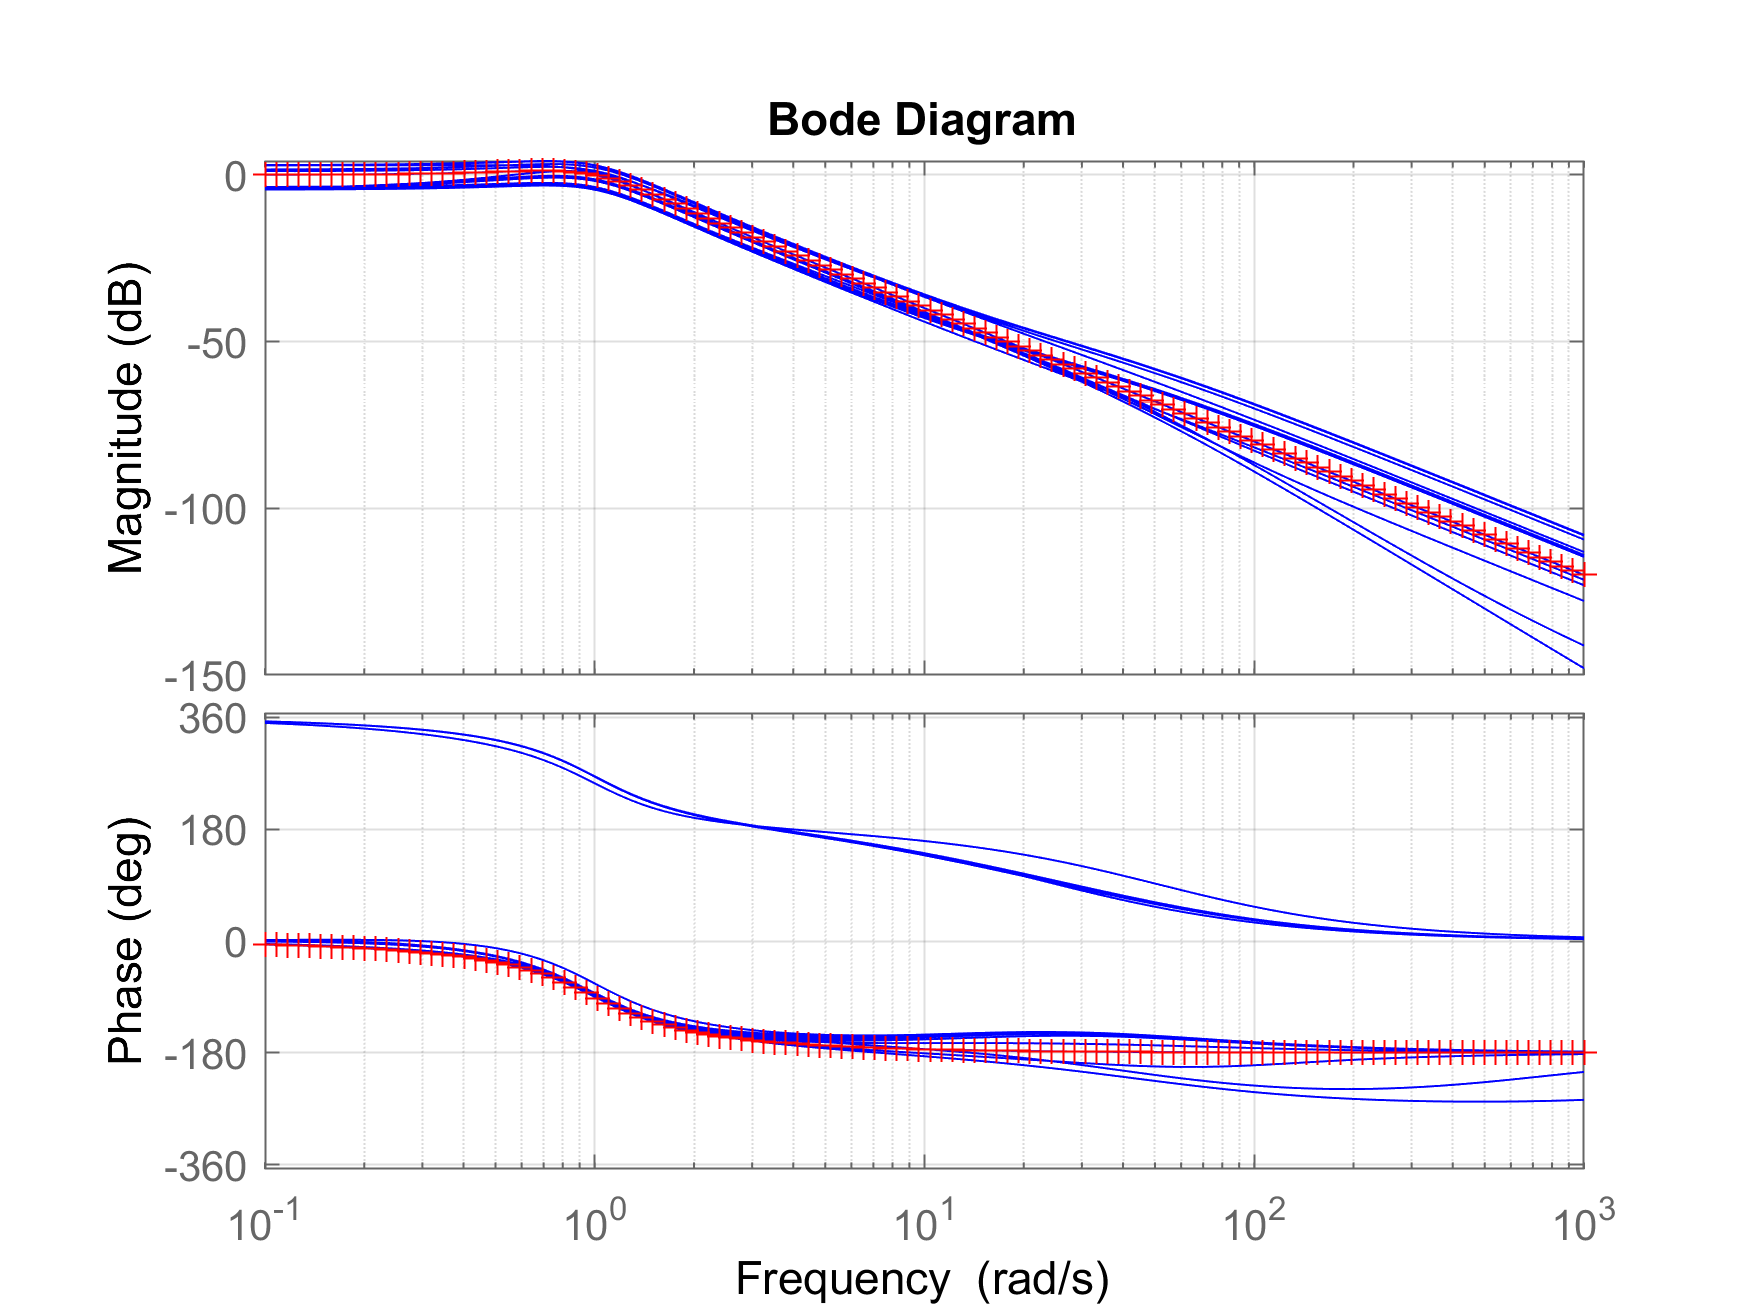
\includegraphics[width=0.6\textwidth]{figures/bode_G.png}
    \caption{}
    \label{fig:bode_G}
\end{figure}

\begin{figure}[H]
    \centering
    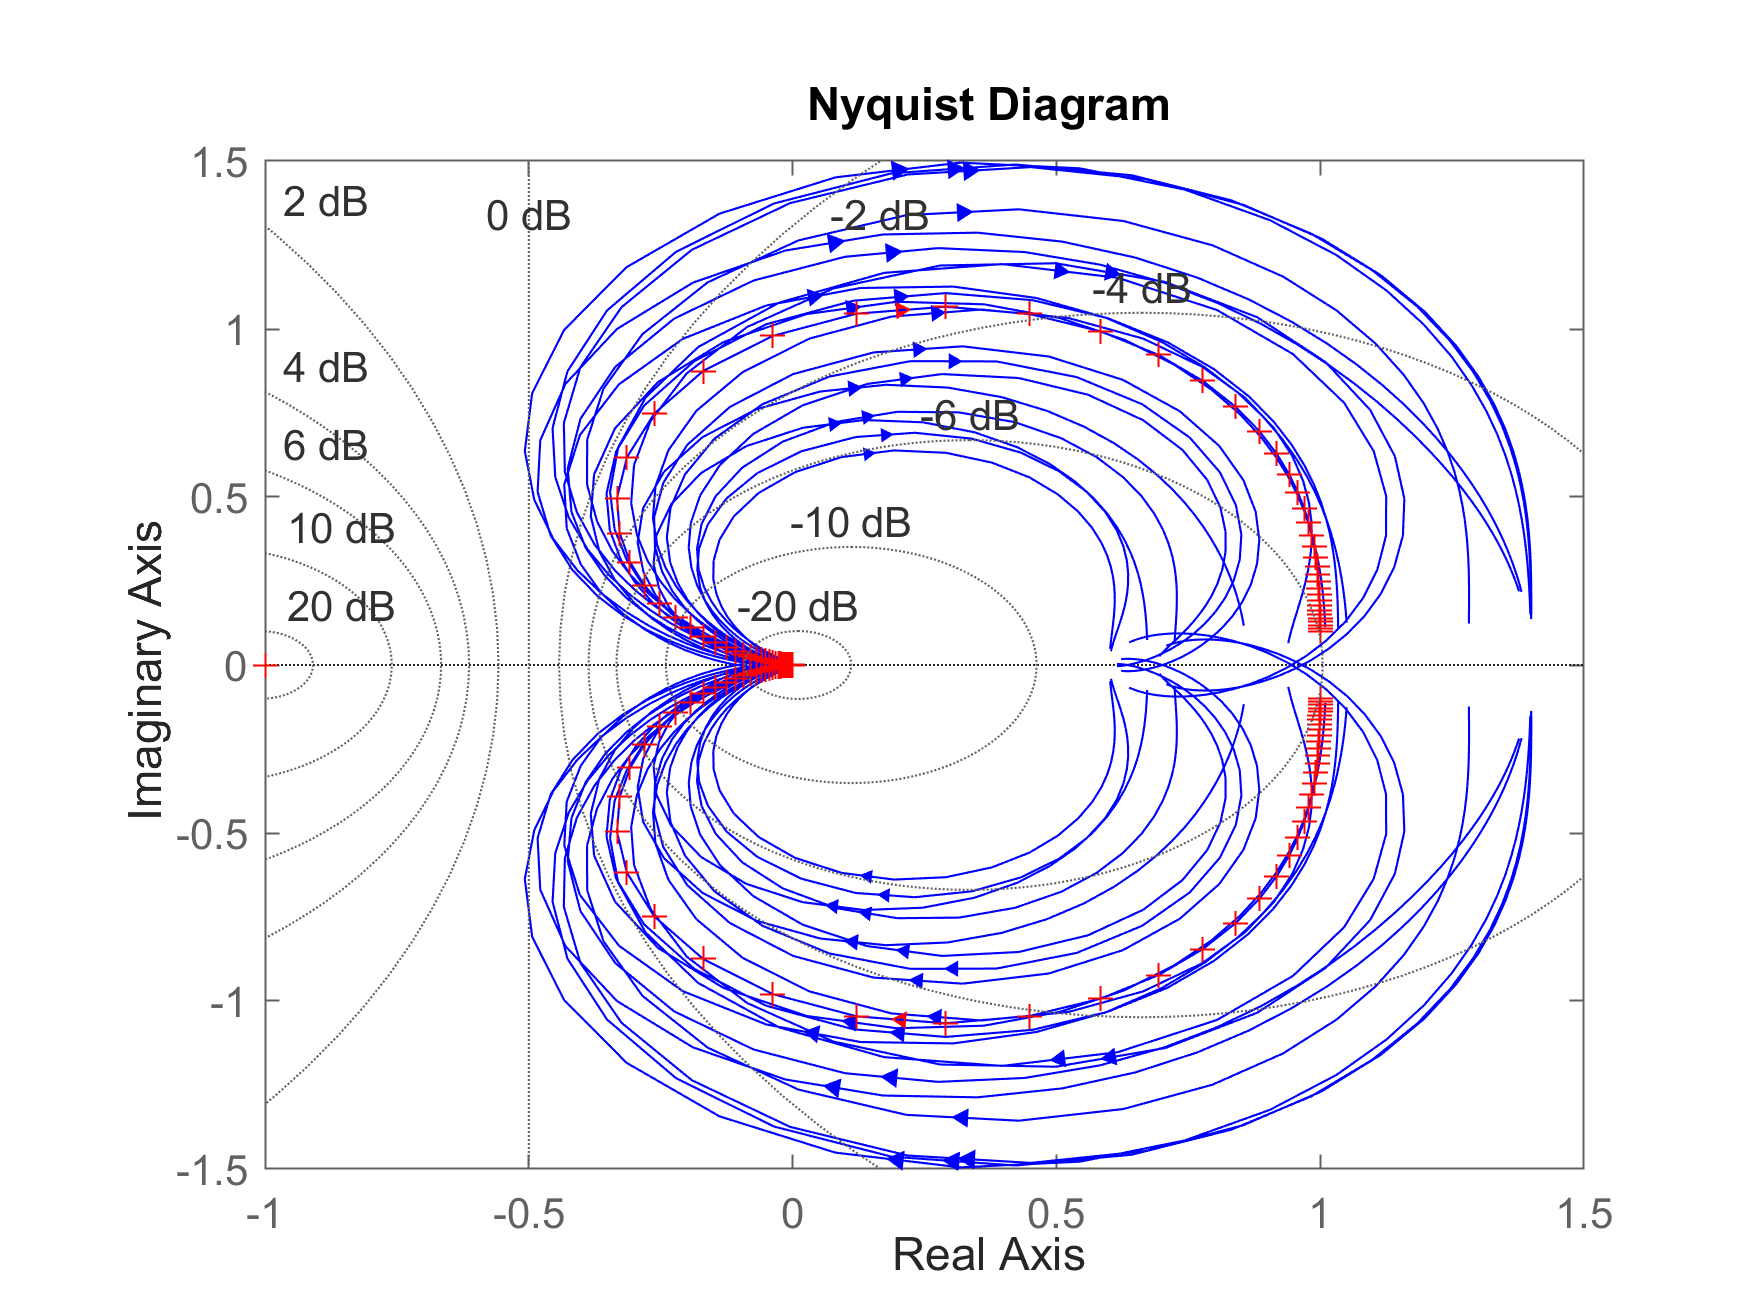
\includegraphics[width=0.6\textwidth]{figures/nyquist_G.png}
    \caption{}
    \label{fig:nyquist_G}
\end{figure}

From the Nyquist plot in figure \ref{fig:nyquist_G} the gain margin is infinite and the phase margin is 90 degrees.

\section{Tracking performance}


The error transfer function of the closed loop is found by evaluating $E(s) = 1/(1+kG(s))$.
For the steady state error to a step response is found by $\frac{1}{s} \cdot E(s)$ and the final value theorem.
\begin{equation}
    \lim_{t \to \infty} e(t) = \lim_{s \to 0} \left( \frac{s}{s} \cdot \frac{\frac{c_p}{m}s^2 + \frac{c_v}{m}s + \frac{c_p}{m}}{s^2 + \frac{c_v}{m}s + (1+k)\frac{c_p}{m}} \right) = \frac{1}{1+k}
\end{equation}
Therefore as $k \to \infty$, the steady state error goes to zero.
This error is also independent of parameters and so should not be affected by uncertainty.

However the damping ratio and frequency are strongly affected by these parameters.
\begin{equation}
    s = \sigma \pm j\omega = -\frac{c_v}{2m} \pm j \frac{1}{2} \sqrt{4(1+k)\frac{c_p}{m} - \left(\frac{c_v}{m}\right)^2}
\end{equation}
\begin{equation}
    \zeta = \frac{-\sigma }{ \sqrt{\sigma^2 + \omega^2}}
\end{equation}

The poles natural frequency is then shown to increase with k, which decreases the damping ratio.
This is also shown graphically on the root locus plot in figure \ref{fig:rlocus_G}.
As $k$ increases, the poles move away from the real axis and the angle between pole and imaginary axis ($\arcsin(\zeta)$) decreases.

\begin{figure}[H]
    \centering
    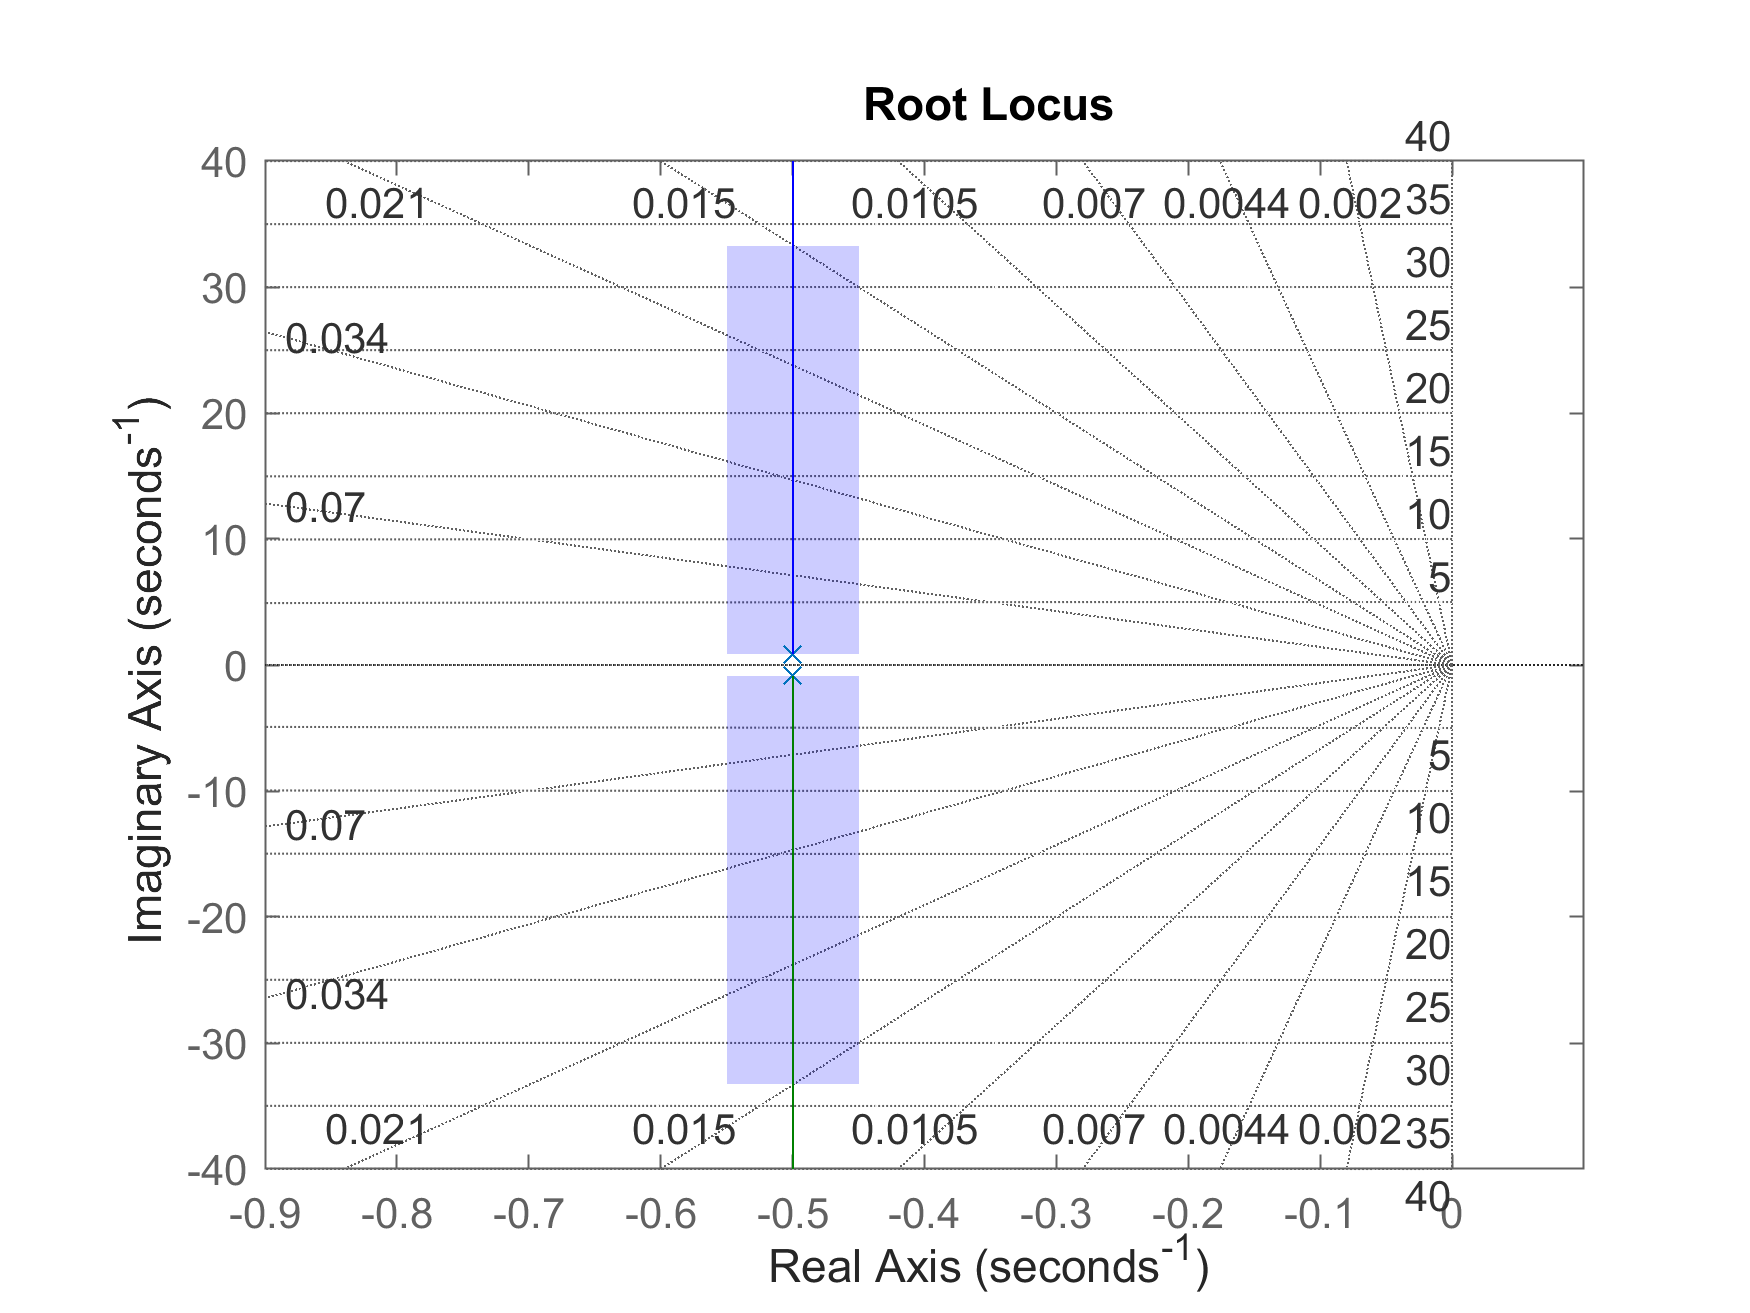
\includegraphics[width=0.6\textwidth]{figures/rlocus_G.png}
    \caption{}
    \label{fig:rlocus_G}
\end{figure}

Figure \ref{fig:rlocus_G} shows the root locus plot for the nominal system for positive values of $k$.
The plot also shows the region of possible pole locations for the parametric uncertainty given in table \ref{tab:parameters}.

\begin{figure}[H]
    \centering
    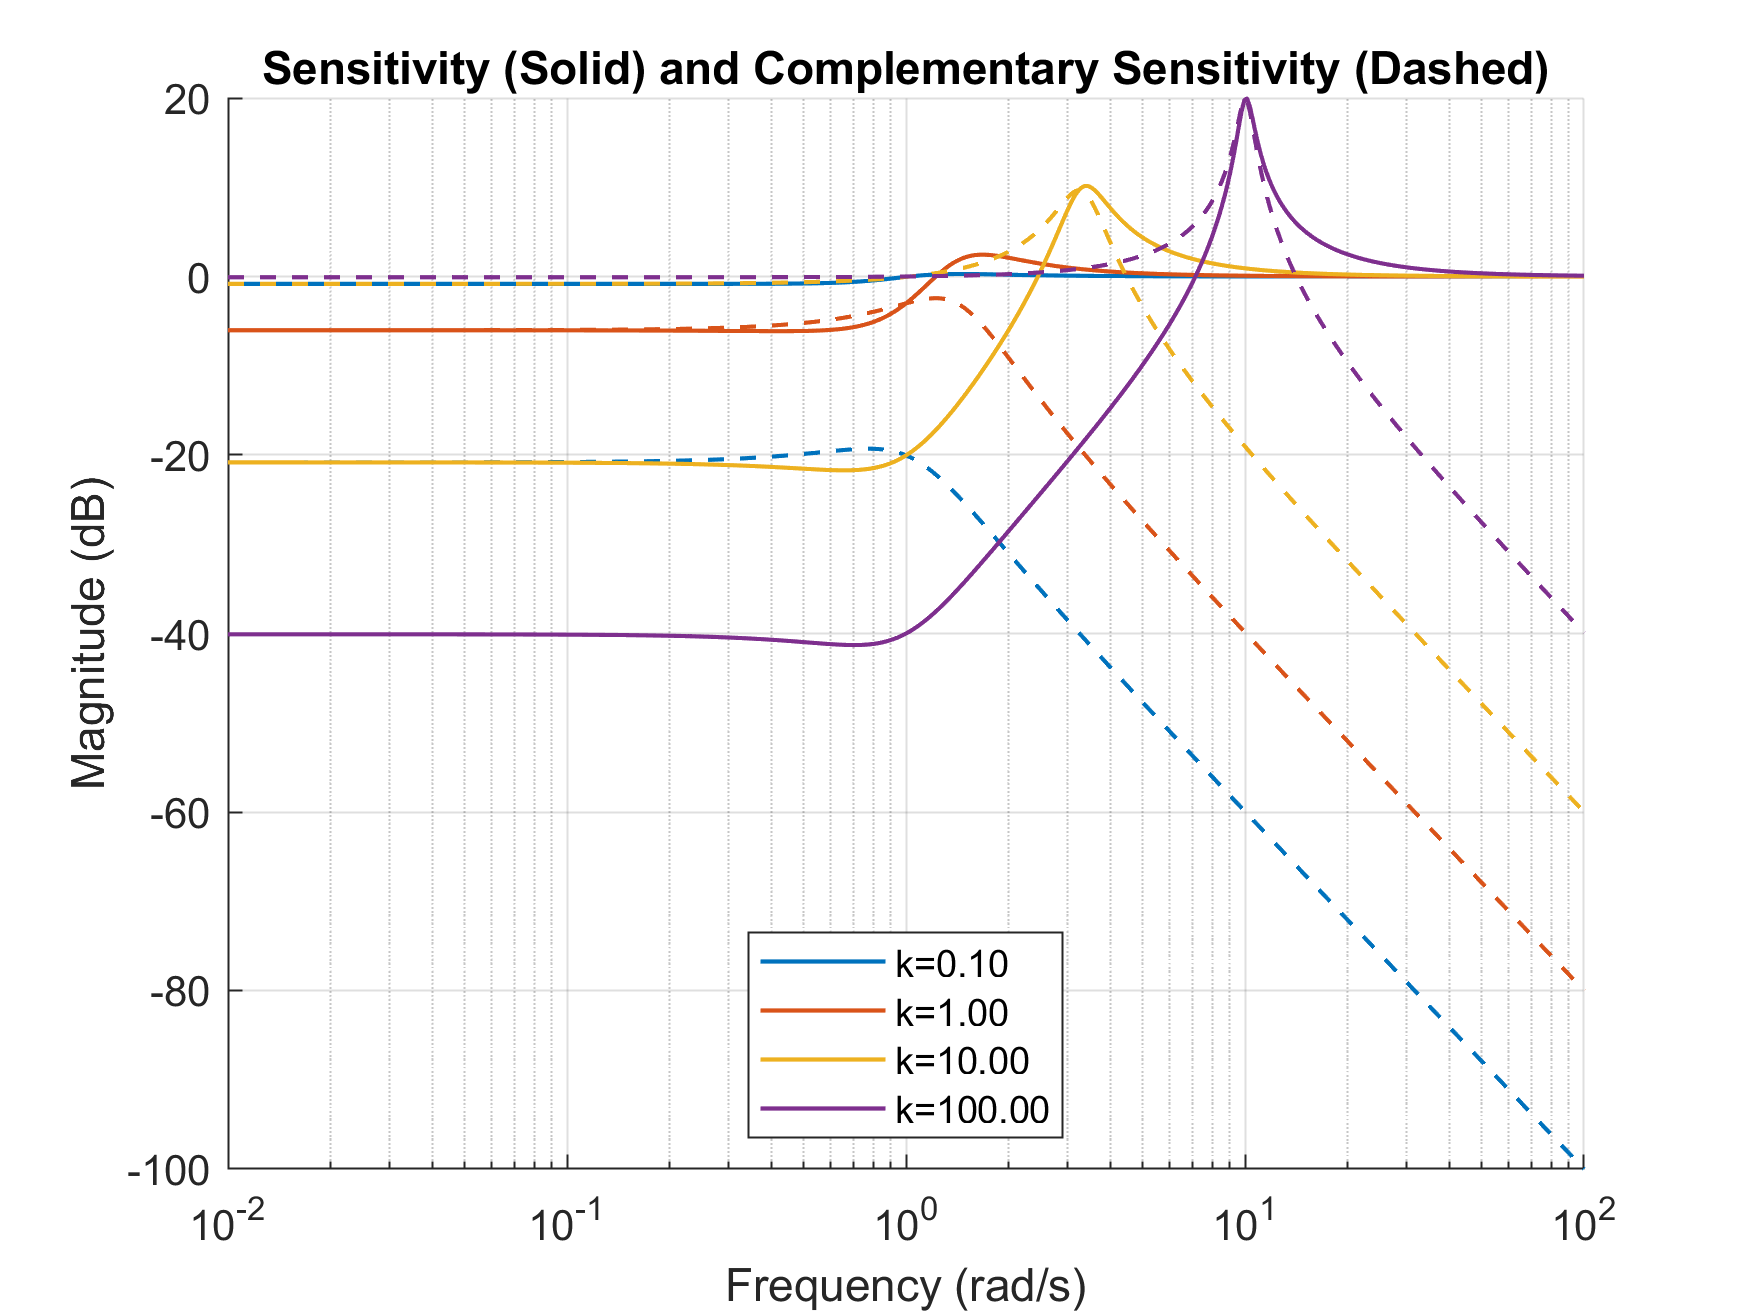
\includegraphics[width=0.6\textwidth]{figures/sensitivities.png}
    \caption{}
    \label{fig:sensitivities}
\end{figure}

Figure \ref{fig:sensitivities} shows the sensitivity and complementary sensitivity response plot for disturbance and reference inputs.
High frequency reference signals are attenuated more by smaller values of $k$. Similarly, high frequency disturbances are amplified less at smaller values of $k$.
At low frequency and small values of k, the sensitivity is higher than the complementary sensitivity which is not desirable.

To gain insight into how parametric uncertainty impacts the system response uncertainty must be propagated as follows:
\begin{equation}
    \delta \omega = \frac{\partial \omega}{\partial c_p} \delta c_p + \frac{\partial \omega}{\partial c_v} \delta c_v \quad \delta \zeta = \frac{\partial \zeta}{\partial c_p} \delta c_p + \frac{\partial \zeta}{\partial c_v} \delta c_v
\end{equation}
The derivatives can be found analytically and are shown plotted against $k$ at otherwise nominal values in figure \ref{fig:u_propagation}.

\begin{figure}[H]
    \centering
    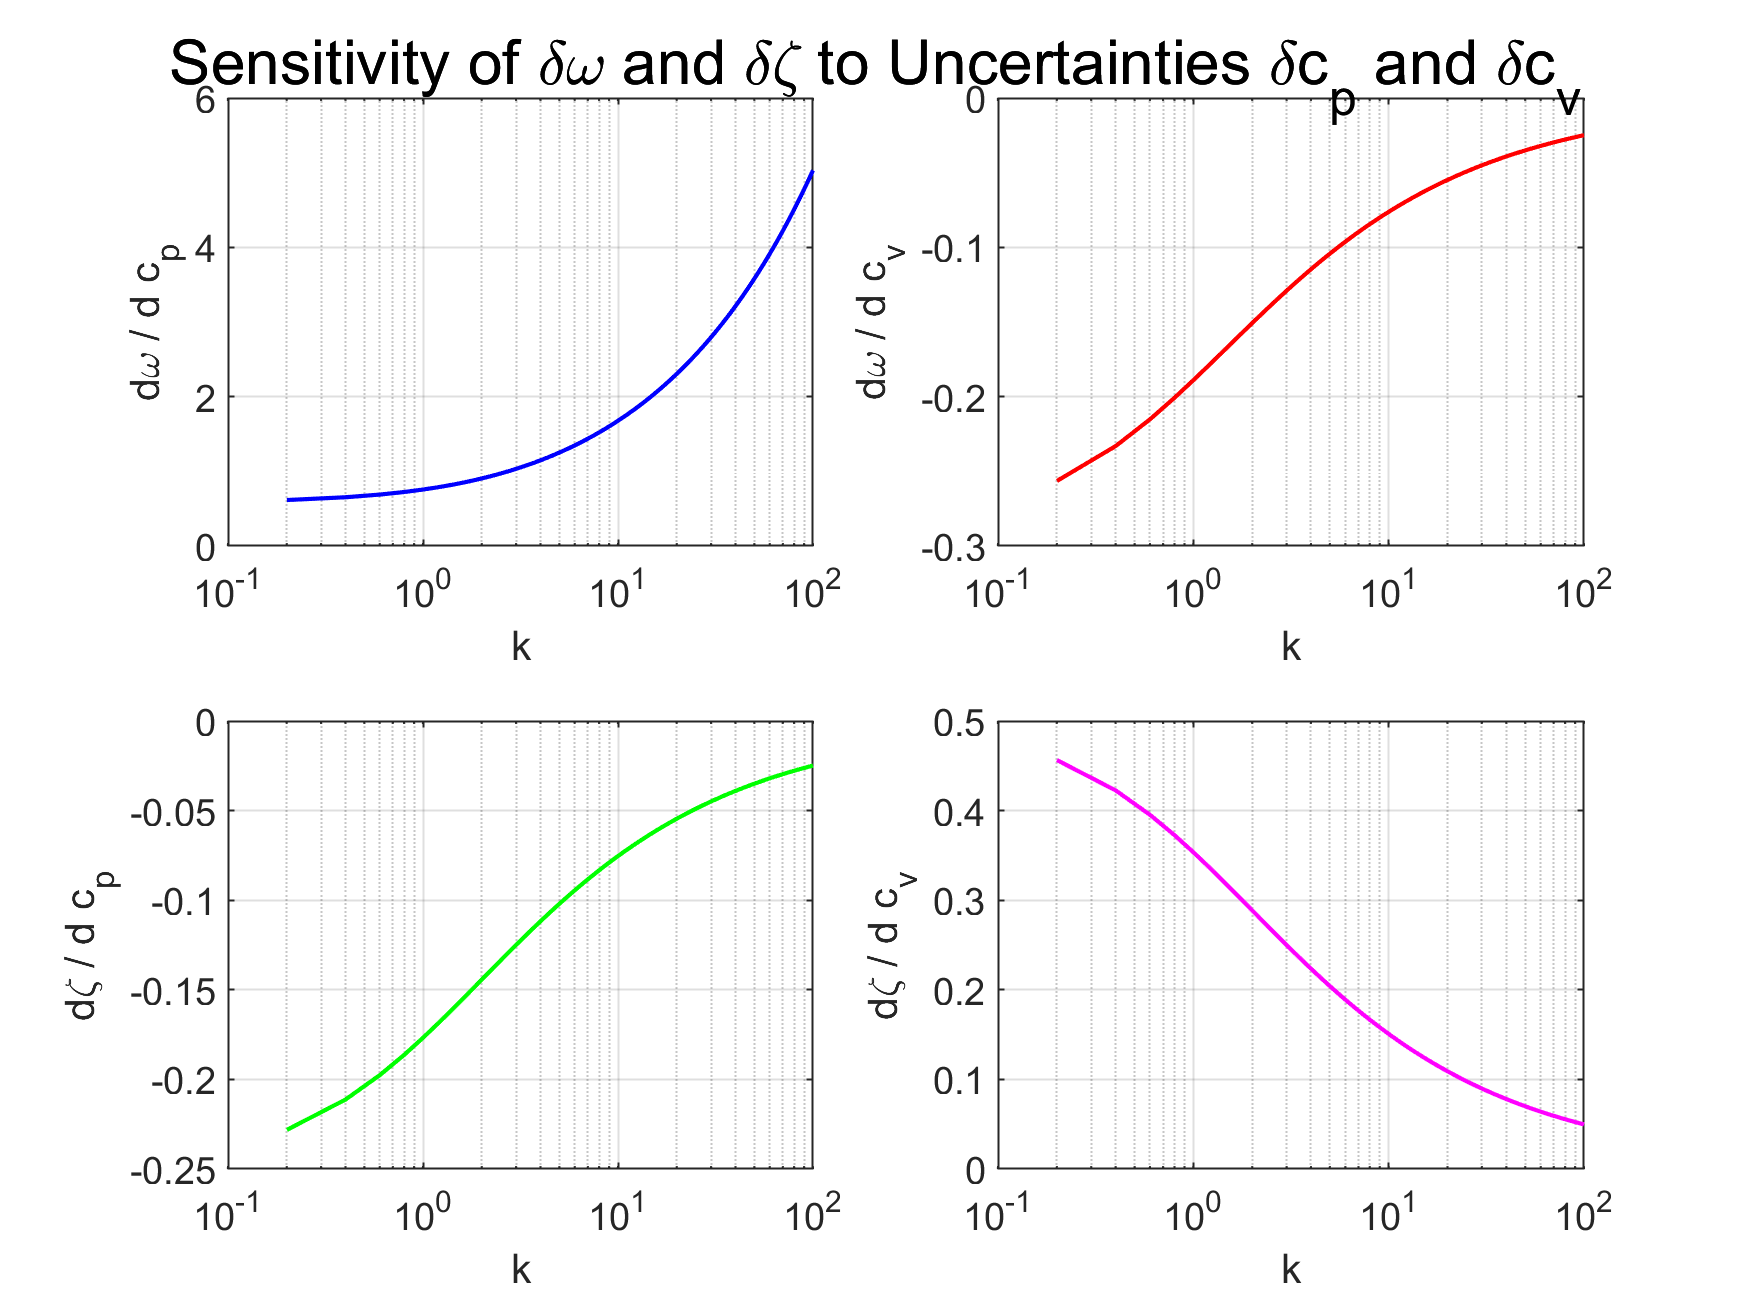
\includegraphics[width=0.6\textwidth]{figures/u_propagation.png}
    \caption{}
    \label{fig:u_propagation}
\end{figure}
Figure \ref{fig:u_propagation} shows how the uncertainty in response parameters changes with $k$.
Small changes in damping ratio due to the parametric uncertainty become less pronounced as $k$ increases.
However, the component of uncertainty in the frequency due to the stiffness coefficient, $c_p$, is shown to increase with $k$.

\begin{thebibliography}{9}

    %Endres, SC, Sandrock, C, Focke, WW (2018) “A simplicial homology algorithm for lipschitz optimisation”, Journal of Global Optimization.
    
      \bibitem{handout}
      J. V. Taylor and J. C. Massey
      \emph{GA3 Heat Exchanger Handout}
      University of Cambridge,
      2024.
    
      \bibitem{HeatTransfer}
      Holman J. P.
      \emph{Heat Transfer. 10th ed.}
      McGraw-Hill,
      2010.
    
      \bibitem{HE_design}
      Sadik Kakac, Hongtan Liu, Anchasa Pramuanjaroenkij,
      \emph{Heat Exchangers: Selection, Rating, and Thermal Design, Third Edition}
      CRC Press,
      2012.
    
      \bibitem{SHGO}
      Endres, SC, Sandrock, C, Focke, WW,
      \emph{A Simplicial Homology Algorithm for Lipschitz Optimisation},
      Journal of Global Optimization,
      2018.
    
\end{thebibliography}

\end{document}